%
%  Kontkat-Daten
%==============================================================================
\chapter{Anhang Richtlinie}

%------------------------------------------------------------------------------
\section{Wichtige Namen, Anschriften und Telefonnummern}
\label{sec:KontaktDaten}

(Diese Seite ist auch als Word-Datei verf�gbar. 
\href{Anhang/KontaktDaten.pdf}{DateinamenReferenz.pdf}\\
{\itshape ich weis nur nicht wie man aus \LaTeX eine Worddatei aufruft}

\vspace*{10mm}
Thema der Bachelor-/Diplom-/Masterarbeit:

Vorname und NAME der Kandidatin bzw. des Kandidaten:\\

Anschrift:\\
  a) Heimatanschrift:\\

	b) Semester-/Wochentagsanschrift:\\

Telefon/Telefax/elektronische Postanschrift (E-Mail):\\


Falls die Abschlussarbeit in einer Firma durchgef�hrt wird:\\
Name der Firma:\\

Anschrift der Firma:\\

Telefon (Zentrale):\\


Name der Betreuerin/des Betreuers in der Firma \\
(mit Titel bzw. Berufsbezeichnung, z. B. Dipl.-Ing.):\\

Ihre/seine Abteilung:\\
Position innerhalb der Firma (z. B. Abteilungsleiter):\\

Telefonisch/per Telefax/�ber elektronische Post zu erreichen unter:\\


%------------------------------------------------------------------------------
\section{Zeit- und Arbeitsplan}
\label{sec:BeispielPlan}
% - - - - - - - - - - - - - - - - - - - - - 
\begin{figure}[!h]
   \begin{center}
   \fbox{
      \includegraphics[width=\textwidth,angle=0]% Achtung pdf muss schon Hochkant sein !
      {anhang/BspTerminplan.pdf}
      }
      \caption{\label{fig:BspPlan}
               Beispiel f�r Zeit- und Arbeitsplan}
   \end{center}
 \end{figure}
 
\clearpage
% - - - - - - - - - - - - - - - - - - - - - 
 \begin{figure}[!h]
   \begin{center}
   \fbox{
      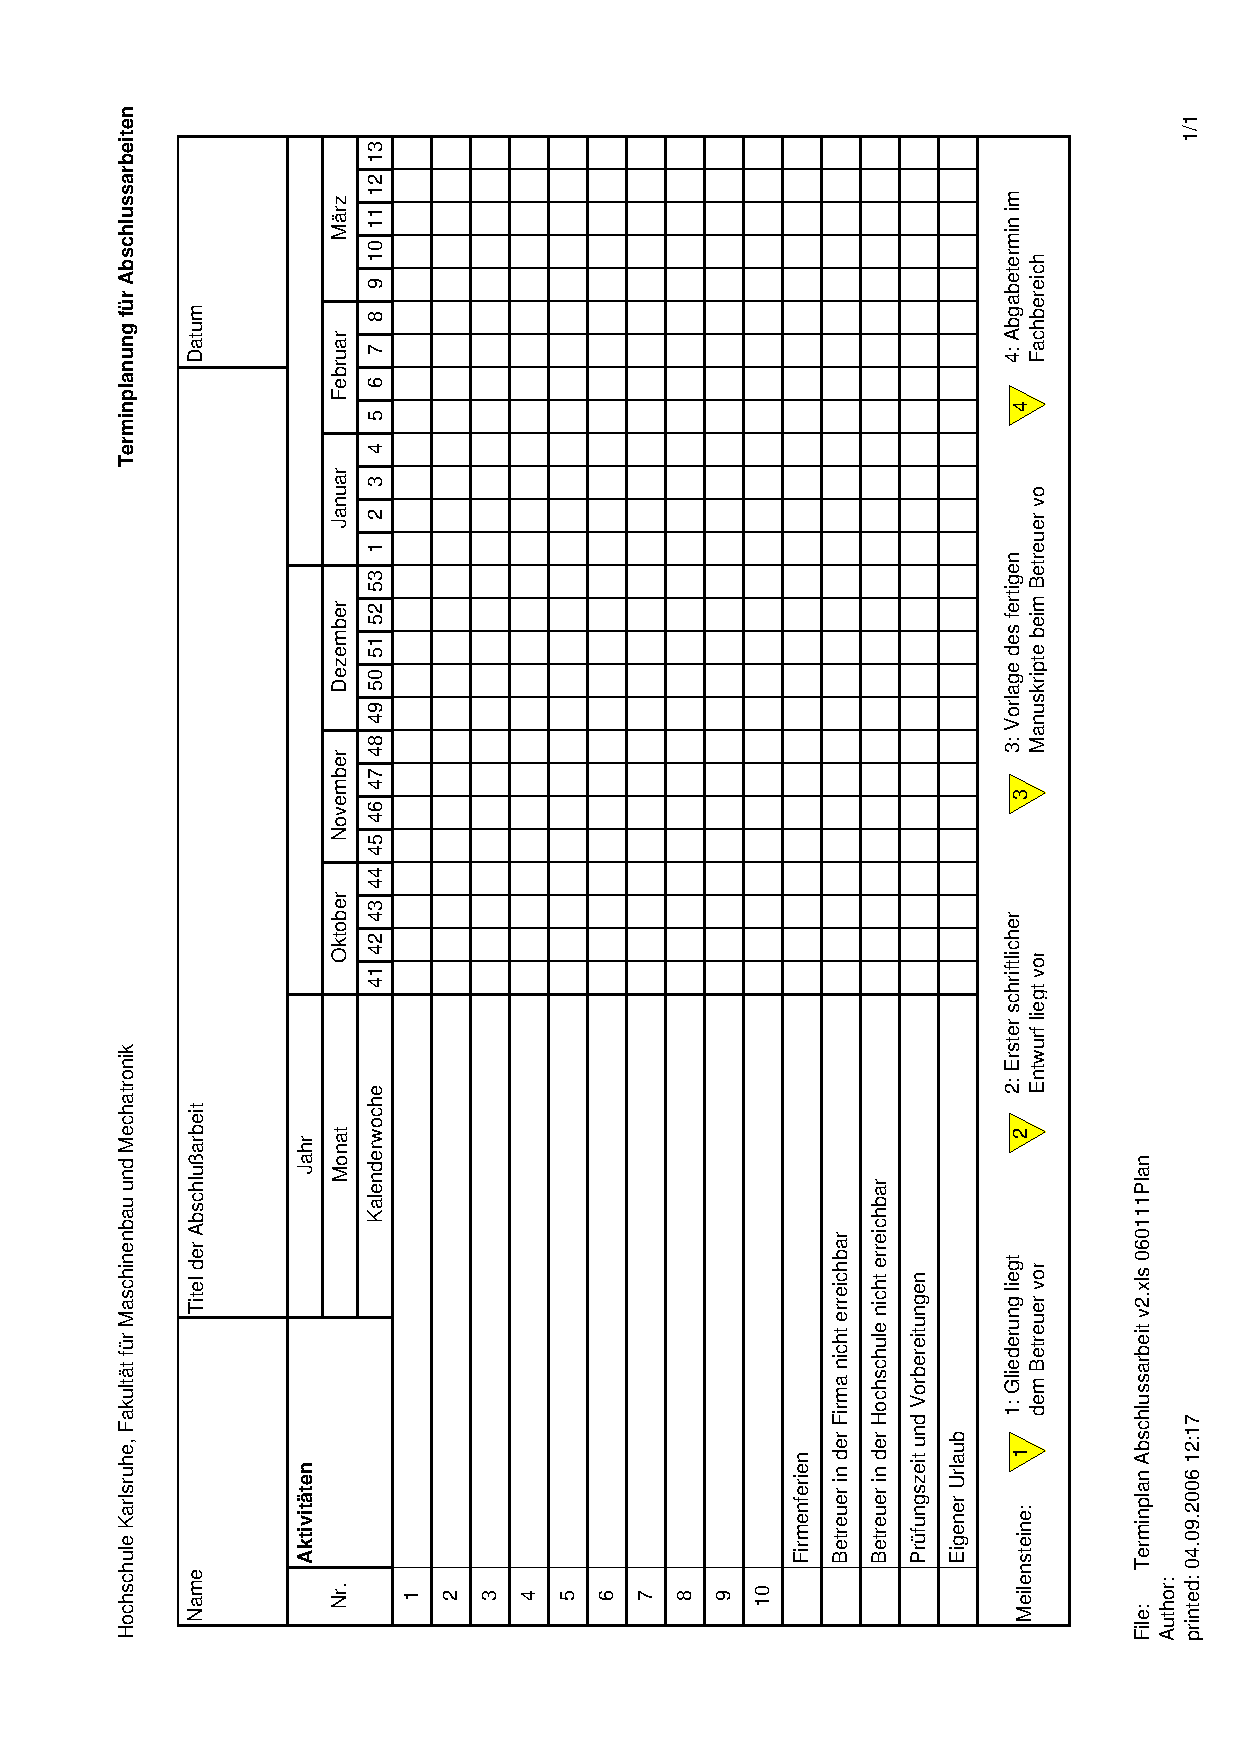
\includegraphics[width=\textwidth,angle=0]
      {anhang/Terminplan_Abschlussarbeit_v2.pdf}
      }
      \caption{\label{fig:Plan}
               Vorlage f�r Zeit- und Arbeitsplan}
   \end{center}
 \end{figure}

\clearpage

%------------------------------------------------------------------------------
\section{Titelseite}
\label{sec:Titelseite}
% - - - - - - - - - - - - - - - - - - - - - 
 \begin{figure}[!h]
   \begin{center}
   \fbox{
      \includegraphics[width=0.85\textwidth, angle=0]{anhang/Titelseite}
      }
      \caption{\label{fig:Titelseite}
               Muster f�r die Titelseite}
   \end{center}
 \end{figure}

\clearpage

%------------------------------------------------------------------------------
\section{Deckblatt}
\label{sec:Deckblatt}

% - - - - - - - - - - - - - - - - - - - - - 
 \begin{figure}[!h]
   \begin{center}
   \fbox{
      \includegraphics[width=0.85\textwidth, angle=0]{anhang/Deckblatt}
        }     
      \caption{\label{fig:Deckblatt}
               Muster f�r das Deckblatt}
   \end{center}
 \end{figure}
 
 \clearpage
 
%------------------------------------------------------------------------------
\section{Erkl�rung und Sperrvermerk}
\label{sec:Erklaerung}
 
% - - - - - - - - - - - - - - - - - - - - -  
 \begin{figure}[!h]
   \begin{center}
   \fbox{
      \includegraphics[width=0.85\textwidth, angle=0]{anhang/Erkl�rung_Sperrvermerk}
        }     
      \caption{\label{fig:Erklaerung}
               Erkl�rung und Beispiel f�r Sperrvermerk}
   \end{center}
 \end{figure}
 
 \clearpage
 
%------------------------------------------------------------------------------
\section{Inhaltsverzeichnis}
\label{sec:Inhaltsverzeichnis}
 
% - - - - - - - - - - - - - - - - - - - - -  
 \begin{figure}[!h]
   \begin{center}
   \fbox{
      \includegraphics[width=0.85\textwidth, angle=0]{anhang/BspInhaltsverzeichnis}
        }     
      \caption{\label{fig:BspInhaltsverzeichnis}
               Beispiel f�r eine Inhaltsverzeichnis}
   \end{center}
 \end{figure}
 
 \clearpage
 
%------------------------------------------------------------------------------
\section{Zusammenfassung}
\label{sec:Zusammenfassung}
 
% - - - - - - - - - - - - - - - - - - - - -  
 \begin{figure}[!h]
   \begin{center}
   \fbox{
      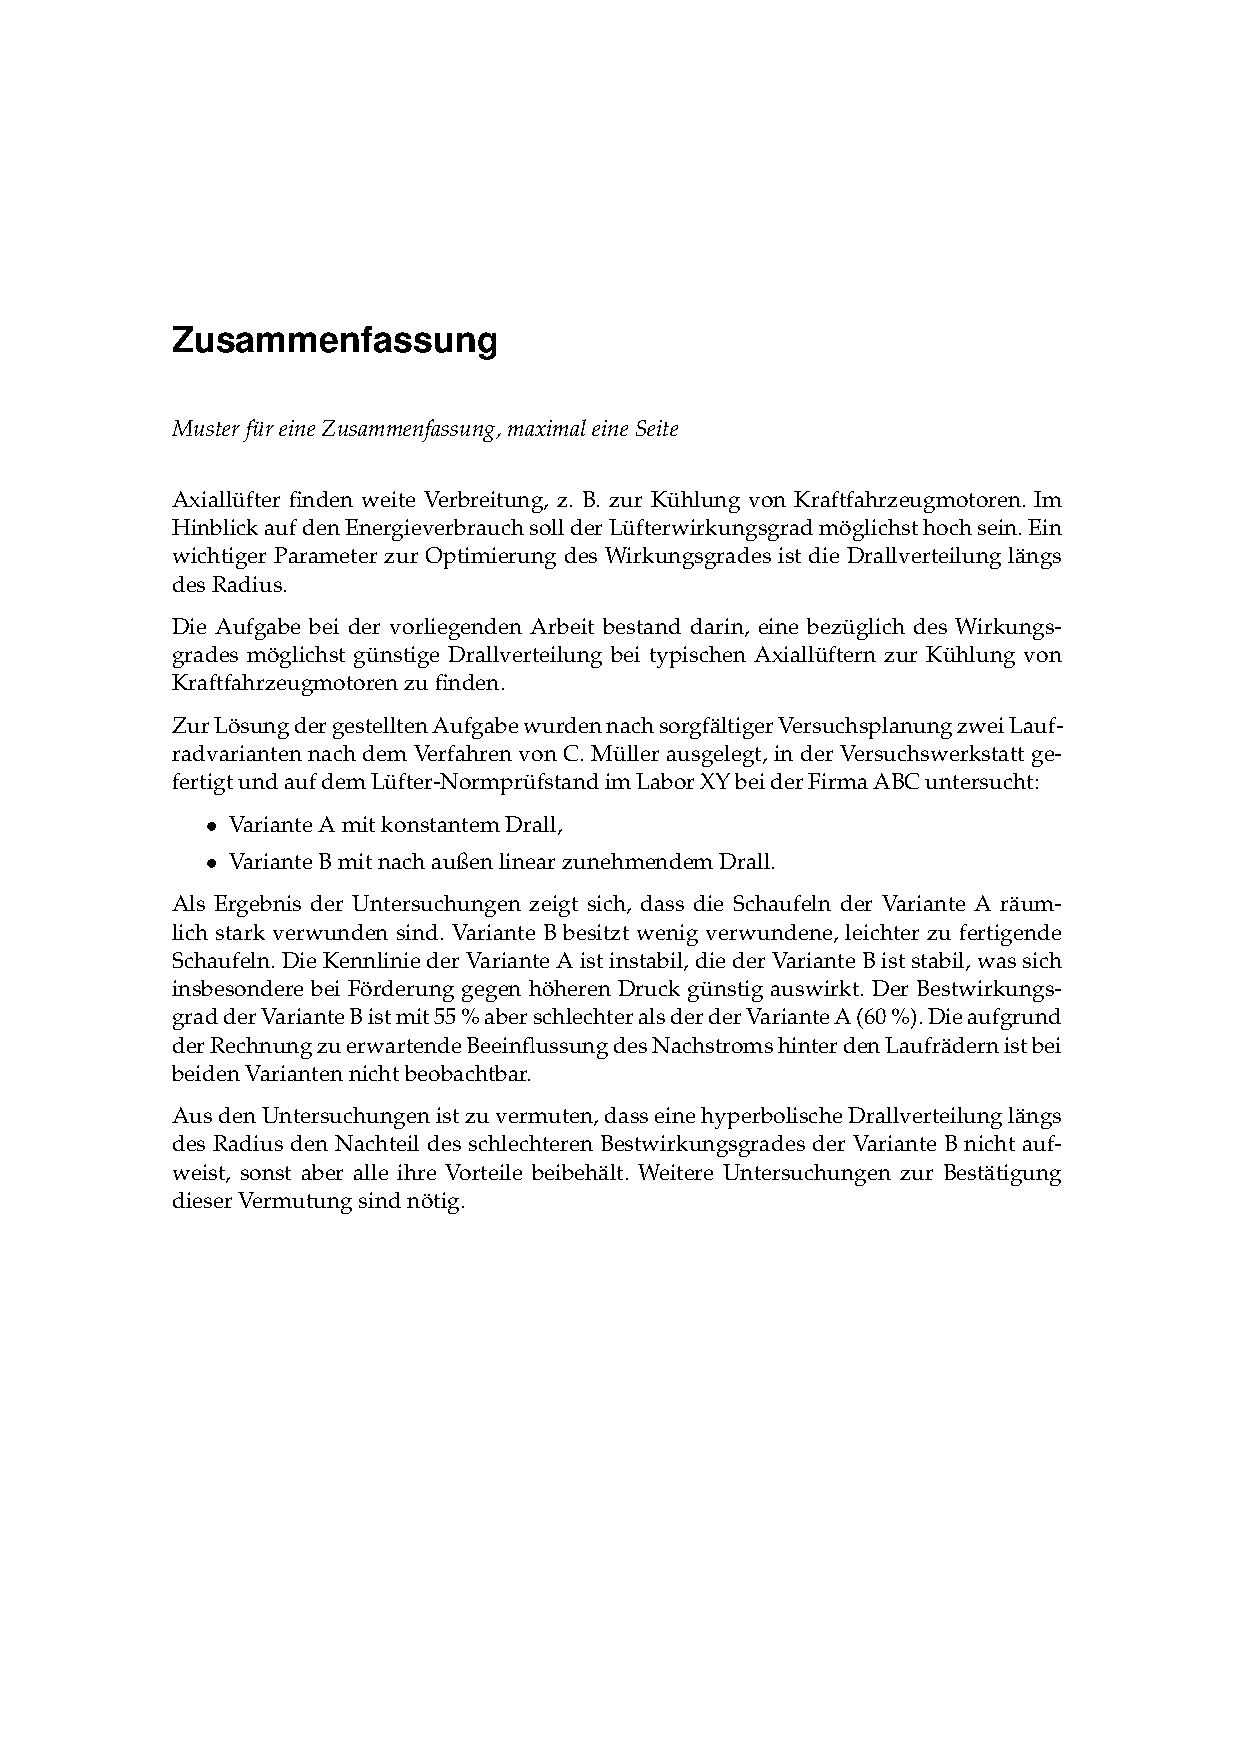
\includegraphics[width=0.85\textwidth, angle=0]{anhang/BspZusammenfassung}
        }     
      \caption{\label{fig:BspZusammenfassung}
               Beispiel f�r eine Zusammenfassung}
   \end{center}
 \end{figure}
 
 \clearpage
 
%------------------------------------------------------------------------------ 
\section{Literaturverzeichnis}
\label{sec:Literaturverzeichnis}
 
% - - - - - - - - - - - - - - - - - - - - -  
 \begin{figure}[!h]
   \begin{center}
   \fbox{
      \includegraphics[width=0.85\textwidth, angle=0]{anhang/BspLitVerzeichnis}
        }     
      \caption{\label{fig:BspLitVerzeichnis}
               Beispiel f�r ein Literaturverzeichnis}
   \end{center}
 \end{figure}
 
 \clearpage
%------------------------------------------------------------------------------   